\section{Model Dynamics}

The dynamics, that emerge from this model, are very similar to the dynamics of the original model described in \Cref{sec:og.dynamics}.
\Cref{fig:final.period.whole.full} displays a 2D scan showing the periods of the stable cycles in the model.
This looks similar to \Cref{fig:yunus.2pi.2d.full}, which is the corresponding 2D scan of the original model.
\Cref{fig:final.period.whole.halved} shows a 2D scan of the halved model, similar to the 2D scans of the halved original model \Cref{fig:yunus.pi.2d.full}.
The reason for scanning the halved model is that we can detect ``type B'' parameter regions this way.
This approach is thoroughly described in \Cref{sec:og.halved}.

\begin{figure}
    \centering
    \begin{subfigure}{0.4\textwidth}
        \centering
        \includegraphics[width=\textwidth]{60_MinimalRepr/2D_Period_Whole_Lotta_Points/result.png}
        \caption{Full Model}
        \label{fig:final.period.whole.full}
    \end{subfigure}
    \begin{subfigure}{0.4\textwidth}
        \centering
        \includegraphics[width=\textwidth]{60_MinimalRepr/2D_Period_Whole_Lotta_Points/result-halved.png}
        \caption{Halved Model}
        \label{fig:final.period.whole.halved}
    \end{subfigure}
    \caption{2D Scans of Periods of Final Model}
\end{figure}

As in \Citeauthor{akyuz2022}'s thesis, we will take a look at the chain of parameter regions, which have stable cycles of period 16.
The parameter regions are marked with the points $A_{16}$ to $G_{16}$.
\Cref{fig:final.cob.start16} shows cobwebs at the start of this chain.
The parameter region containing $A_{16}$ is denoted $\P_{\A^7\B\C^7\D}$ since its only stable cycle is $\Cycle{\A^7\B\C^7\D}$.
This stable cycle can be seen in \Cref{fig:final.cob.A16}.
The parameter region, therefore, is a ``type A'' parameter region with only one stable cycle of period 16.
The next parameter region contains the point $B_{16}$ and has two stable cycles $\Cycle{\A^7\B\C^6\D^2}$ and $\Cycle{\A^6\B^2\C^7\D}$ that \Cref{fig:final.cob.B16} depicts.
Therefore it is denoted $\P_{\A^7\B\C^6\D^2, \A^6\B^2\C^7\D}$.
Per the same logic, the parameter region containing $C_{16}$ is denoted $\P_{\A^6\B^2\C^6\D^2}$.
Its stable cycle can be seen in \Cref{fig:final.cob.C16}.

\begin{figure}
    \centering
    \begin{subfigure}{0.3\textwidth}
        \centering
        \includegraphics[width=\textwidth]{60_MinimalRepr/Cobweb_A16/result.png}
        \caption{Point $A_{16}$}
        \label{fig:final.cob.A16}
    \end{subfigure}
    \begin{subfigure}{0.3\textwidth}
        \centering
        \includegraphics[width=\textwidth]{60_MinimalRepr/Cobweb_B16/result.png}
        \caption{Point $B_{16}$}
        \label{fig:final.cob.B16}
    \end{subfigure}
    \begin{subfigure}{0.3\textwidth}
        \centering
        \includegraphics[width=\textwidth]{60_MinimalRepr/Cobweb_C16/result.png}
        \caption{Point $C_{16}$}
        \label{fig:final.cob.C16}
    \end{subfigure}
    \caption{Cobwebs of the Start of Period 16 Chain in Final Model}
    \label{fig:final.cob.start16}
\end{figure}

Thus far these parameter regions follow the rules laid out in \Citeauthor{akyuz2022}'s thesis~\Cite{akyuz2022}.
The first parameter region has the stable cycle $\Cycle{\A^{\frac{P}{2} - 1}\B\C^{\frac{P}{2} - 1}\D}$ where $P = 16$ is the period.
It is a ``type A'' parameter region and the next parameter region is of ``type B'', as the rules require.
This parameter region has the stable cycles $\Cycle{\A^{\frac{P}{2} - 1}\B\C^{\frac{P}{2} - 2}\D^2}$ and $\Cycle{\A^{\frac{P}{2} - 2}\B^2\C^{\frac{P}{2} - 1}\D}$.
This also agrees with the rules.
The next parameter region is of ``type A'' again and has the stable cycle $\Cycle{A^{\frac{P}{2} - 1}\B^2\C^{\frac{P}{2} - 2}\D^2}$ as expected by the rules.
This chain continues to abide by the rules as can be seen in the cobwebs of points $D_{16}, E_{16},$ and $F_{16}$ in \Cref{fig:final.cob.mid16}.
The corresponding parameter regions are $\P_{\A^6\B^2\C^5\D^3, \A^5\B^3\C^6\D^2}, \P_{\A^5\B^3\C^5\D^3},$ and $\P_{\A^5\B^3\C^4\D^4, \A^4\B^4\C^5\D^3}$ respectively.

\begin{figure}
    \centering
    \begin{subfigure}{0.3\textwidth}
        \centering
        \includegraphics[width=\textwidth]{60_MinimalRepr/Cobweb_D16/result.png}
        \caption{Point $D_{16}$}
        \label{fig:final.cob.D16}
    \end{subfigure}
    \begin{subfigure}{0.3\textwidth}
        \centering
        \includegraphics[width=\textwidth]{60_MinimalRepr/Cobweb_E16/result.png}
        \caption{Point $E_{16}$}
        \label{fig:final.cob.E16}
    \end{subfigure}
    \begin{subfigure}{0.3\textwidth}
        \centering
        \includegraphics[width=\textwidth]{60_MinimalRepr/Cobweb_F16/result.png}
        \caption{Point $F_{16}$}
        \label{fig:final.cob.F16}
    \end{subfigure}
    \caption{Cobwebs of the Middle of Period 16 Chain in Final Model}
    \label{fig:final.cob.mid16}
\end{figure}

Scanning the periods of this model for larger $p_y$ values, we see the ends of the chains.
\Cref{fig:final.period.end.full} shows the scan of the full model and \Cref{fig:final.period.end.halved} for the halved model, indicating the ``type B'' parameter regions.
For the chain of period 16, the ``type B'' parameter region $\P_{\A^3\B^5\C^2\D^6, \A^2\B^6\C^3\B^5}$ is missing from this chain, it would have been marked with the point $J_{16}$.
And the last parameter region is the parameter region containing the point $K_{16}$, $\P_{\A^2\B^6\C^2\D^6}$.
The missing ``type B'' parameter region violates the rule, that a chain always alternates between parameter regions of ``type B'' and ``type A''.
Also, the last parameter region is not $\P_{\A\B^7\C\D^7}$, as the rules predicted.
Instead, the parameter region containing $K_{16}$, which is the last parameter region, is $\P_{\A^2\B^6\C^2\D^6}$.
In \Citeauthor{akyuz2022}'s thesis, the last parameter region for the chain of period 16 was also $\P_{\A^2\B^6\C^2\D^6}$~\Cite{akyuz2022}.

\begin{figure}
    \centering
    \begin{subfigure}{0.4\textwidth}
        \centering
        \includegraphics[width=\textwidth]{60_MinimalRepr/2D_Period_Chain_Ends/result.png}
        \caption{Full Model}
        \label{fig:final.period.end.full}
    \end{subfigure}
    \begin{subfigure}{0.4\textwidth}
        \centering
        \includegraphics[width=\textwidth]{60_MinimalRepr/2D_Period_Chain_Ends/result-halved.png}
        \caption{Halved Model}
        \label{fig:final.period.end.halved}
    \end{subfigure}
    \caption{2D Scans of Periods of Final Model Showing the End of the Chains}
\end{figure}

But when we go beyond the ``end'' of the chain, we find a parameter region $\P_{\A\B^7\C\D^7}$ at higher $p_y$ values.
It is marked with the point $M_{16}$ in \Cref{fig:final.period.beyond.full} and \Cref{fig:final.period.beyond.halved}.
The higher period region below the period region $\P_{\A\B^7\C\D^7}$ region that indicates a possible ``type B'' parameter region is not the parameter region $\P_{\A^2\B^5\C\D^7, \A\B^7\C^2\D^5}$ but rather $\P_{\A^2\B^4\C\D^7, \A\B^7\C^2\D^4}$.
Incidentally, the parameter region $\P_{\A^2\B^4\C^2\D^4}$ is just below this parameter region.

\begin{figure}
    \centering
    \begin{subfigure}{0.4\textwidth}
        \centering
        \includegraphics[width=\textwidth]{60_MinimalRepr/2D_Period_Chain_Ends_Cont/result.png}
        \caption{Full Model}
        \label{fig:final.period.beyond.full}
    \end{subfigure}
    \begin{subfigure}{0.4\textwidth}
        \centering
        \includegraphics[width=\textwidth]{60_MinimalRepr/2D_Period_Chain_Ends_Cont/result-halved.png}
        \caption{Halved Model}
        \label{fig:final.period.beyond.halved}
    \end{subfigure}
    \caption{2D Scans of Periods of Final Model Beyond the Chains}
\end{figure}
